\chapter{Fenix Framework}
\label{chap:ff}

``Fenix Framework allows the development of Java-based applications
that need a {\it transactional and persistent domain model.}''

This chapter describes in detail the major components of the Fenix
Framework, used to implement the solution proposed throughout this
document. Section \ref{sec:dml} describes the Domain Modelling
Language, used to describe the application's domain model. Section
\ref{sec:ff-arch} describes the high-level architecture of the
Framework, briefly describing its major components and their
interaction. Section \ref{sec:jvstm} presents the Java Versioned STM
(JVSTM), and its integration with the Fenix Framework. The information
presented in this chapter is critical to understanding the proposed
solution, as well as its challenges.

\section{Domain Modelling Language}
\label{sec:dml}

The Fenix Framework is aimed at entreprise-class applications with a
rich domain model in an object-oriented paradigm. Such applications
typically consist of class hierarchies representing entities with
relationships among them, forming an interconnected graph. 

The Domain Modelling Language (DML) is a Domain-Specific Language
designed to represent such domain models, separating the domain's
structure from its behaviour. The DML is designed with modularity as a
core concern, allowing for incremental and modular domain definition.

In a DML file, programmers write their domain definition in a
Java-like language. A class definition consists of the class name, the
persistent slots (either primitive or value types), and the
super-class. Listing \ref{list:class-example} shows how the {\it
  Course} class from Figure \ref{fig:courseDomain} could be described
in the DML. Note that as arrays are not natively supported, a Value
Type must be created, describing an array of publications. Value Types
are described in more detail below.

\begin{lstlisting}[caption={DML for the {\it Course} and {\it
      Department} classes},
  label={list:class-example}]
class Course {
  String name;
  String objectives;
  int credits;
  PublicationList bibliography;
}

class Department {
  String name;
}
\end{lstlisting}

Relations in DML are named, first-class entities which represent
relationship between two classes. Relations are always bi-directional,
meaning that updating one side of the relation will automatically
update the other side. Relations can be concealed in one of the sides
(meaning that it will not be possible to access it), however their
state is still kept.

It is possible to define {\it one-to-one}, {\it one-to-many} and {\it
  many-to-many relationships}, and it is possible to define boundaries
on the multiplicity of each relation (for example, a {\it Department} can
have between 0 and 30 {\it Courses}. Any violation to these
constraints will put the relation in an inconsistent state and will be
discarded. 

To-Many relations in the Fenix Framework have Set semantics, meaning
that an object can only be present in a relation once. Also, there are
no ordering guarantees when accessing the relation.

\begin{lstlisting}[caption={DML for the relation between {\it Course}
    and {\it Department}},label={list:relation-example}]
relation DepartmentHasCourses {
  Department playsRole department {
    multiplicity 1..1;
  }
  Course playsRole course {
    multiplicity *;
  }
}
\end{lstlisting}

Listing~\ref{list:relation-example} shows how the relation presented
in Figure~\ref{fig:courseDomain} could be described in the DML. The
relation is given a name that accurately describes the ownership
relation between the two classes, as well as names to describe the
role of each class. The multiplicity is defined for each of the roles,
in this case, one {\it Department} has zero or more {\it Courses}, and
one {\it Course} has between one and one (exactly one) {\it
  Department}.


From the domain definition, the Fenix Framework generates Java getters
and setters for the properties and relations. For each DML class, a
Java class is created, along with a {\it Base} class, containing the
generated methods, as well as internal helper methods used to persist
the properties. As such, Base classes contain the application's
structure, and the non-Base classes contain the application's
behaviour. Generation of base classes is described in more detail in
Section~\ref{sec:codeGen}.

\subsection{Value Types}

In the DML there is a distinction between entities (classes and
relations) and value objects. Whereas an entity is transactional and
persistent, a value object is immutable and not persistent. Value
objects are used as the values for slots of DML classes, and must be
of well-known types, known as Value Types.

A value type contains information regarding the Java Type (such as
{\it java.math.BigDecimal}), an alias (such as {\it BigDecimal}), and information
regarding how the object will be externalised/internalized. 

There are two categories of Value Types: Builtin (Java Primitives and
their wrappers, Enums, JodaTime types, JsonElement, and byte arrays)
and user-defined. User-defined types allow the programmer to use any
type they wish as a slot, provided the type is immutable (explanation
as to why is provided ahead) and can be expressed in terms of other
Value Types.

The Framework knows how to handle Builtin Value Types (i.e. how to
store/retrieve from persistent support). User-defined, on the other
hand, require that the programmer specify how the type is
externalised/internalized. The externalised type must be either a
Builtin Value Type, or a used-defined one (provided it externalises to
a builtin).

\subsection{JSON}

JSON (JavaScript Object Notation) is described as being ``[...] a
lightweight data-interchange format.''. JSON is quickly becoming the
de-facto standard to interchange data across heterogeneous systems,
replacing XML in many cases.

As such, in the context of this work, the Framework was extended to
provide native JSON support (by allowing it as a Builtin Value Type),
using Google's GSON\footnote{http://code.google.com/p/google-gson/}.
Using JSON allows the programmer to define arbitrarily complex Value
Types with little effort, as well as simplifying externalisation code.

The Framework also provides support to transform any Value Type
to/from JSON, meaning that a JsonElement slot is enough to keep any
value the Fenix Framework is able to handle. As will be presented in
Chapter~\ref{chap:solution}, this proves to be a crucial feature.

\section{Architecture}
\label{sec:ff-arch}

In Fenix Framework 1.x (as presented in \cite{fernandes2011strict})
had a rather monolithic architecture. Transactional support was
provided by the JVSTM (see Section \ref{sec:jvstm}), and persistence
was implemented on top of MySQL, leaving the programmer with no other
choice of technology.

With the second major version of the Framework (released earlier this
year), a great architectural shift has occurred. There is now a clear
separation between the Framework's public API and the
transactional/persistence backends, allowing for a ``write once, run
everywhere'' paradigm. The programmer simply writes his application
against a public API and is able to run it on multiple backends.

This way, not only are applications portable across several
technologies (MySQL, Neo4j, MongoDB, etc), but also testing support is
greatly enhanced, as there is no need to mock the persistence API, as
tests can be run using an in-memory backend.

Figure~\ref{fig:ff-arch} shows the major modules that constitute the Fenix
Framework.

\begin{figure}
\centering
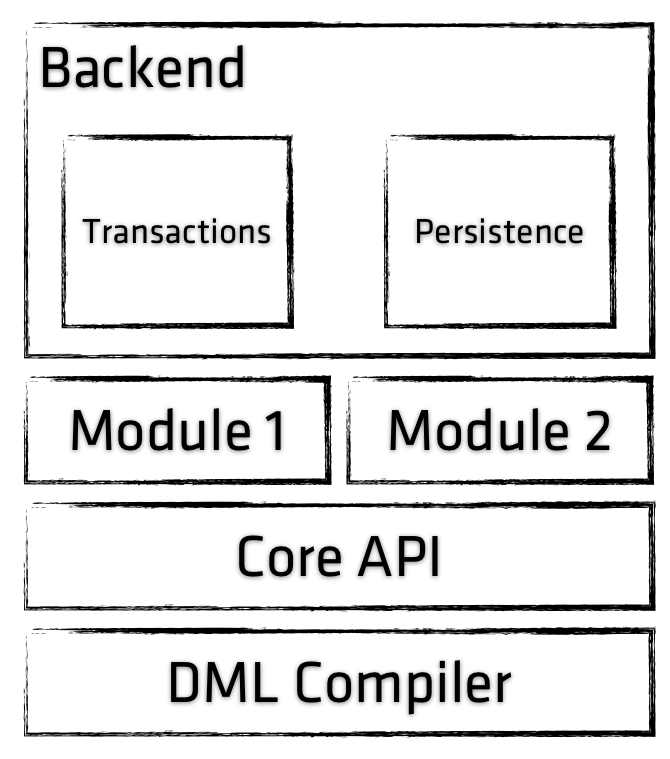
\includegraphics[width=0.5\linewidth]{ff-arch}
\caption{Fenix Framework Architecture}
\label{fig:ff-arch}
\end{figure}

The 'DML Compiler' module contains the parser responsible for reading
DML files and creating an in-memory description of the Domain Model,
as well as all the necessary classes to represent it. It also contains
the base {\it DomainObject} interface, which all objects of the Domain
Model implement. Also present in this module are the base Code
Generators used to create the Base classes for all domain
objects.

The core of the Framework is in the 'Core API' module. Transaction
management APIs, configuration, entry points, backend interfaces, are
all defined in this module.

Many backend-independent modules are provided with the Fenix Framework
bundle. These include persistent Abstract Data Types (B+Trees, Linked
Lists, etc), support for Consistency
Predicates \cite{JoaoCoutinhoNeves2011}, statistics collection tools,
indexing and transaction introspection. These modules are used
internally by the various backends, but can (and in most cases should)
also be used by the programmers.

Backends provide the concrete implementations of transactional and
persistence support, and are required for applications to work.

\subsection{Public API}

One of the major advantages of the Fenix Framework is that
applications built on top of it are independent of the underlying
persistence and transactional backend. However, to guarantee this
property, the modules that form the such applications must be compiled
against the Public API of the Framework.

The public API is split in two major components:

\begin{itemize}
\item {\bf DML Compiler} Allows applications to have runtime access to
  the structure of the domain and allows registering relation
  listeners that will be invoked each time a relation is
  modified. This module also defines the API that is generated based
  on the DML, which must be supported by all backends.

\item {\bf Core API} Provides the entry point for the domain's object
graph through the {\it DomainRoot} class, the mechanism to retrieve a
Domain Object from its unique identifier, transaction APIs that can be
used to either mark a piece of code as transactional (@Atomic
annotation) or to manually manage the lifecycle of transactions and
utilities to configure the Framework.
\end{itemize}

With this separation the classpath of the application modules is not
'polluted' with implementation details, allowing for a faster
development and test cycle.

\subsection{Backends}

Backends provide concrete implementations of the transactional and
persistence support. Application modules should not depend directly on
the backends, as their API is private and as such subject to change
even among minor versions, and having a dependency on a specific
backend means that portability must be sacrificed.

The fact that backends have a clear separation from the Public API
allows for a much faster evolution of the backend's
implementation. Major internal changes can be done without affecting
the end-users directly, even in a revision release, whereas changes to
the public API require either a major or minor release. 

COMPLETE

\section{Code Generation}
\label{sec:codeGen}

In the Fenix Framework, access to persistent fields is done through
generated methods in Base classes. 

There are two major components in code generation:

\begin{itemize}

\item The default code generator, from which every other generator
  inherits, defines the public generated API for domain classes. Its
  major use-case is to compile backend agnostic application modules
  that only need base classes because of their API (modules aren't
  bundled with base classes, those are generated on-demand on
  depending modules or applications).

\item Backend-provided code generators. These generators extend the
  base ones, thus providing the same API, using backend-specific
  artifacts to fullfil the API. Backends can also use code generators
  to optimise runtime performance, by injecting in generated code
  values that otherwise would have to be computed in runtime.
\end{itemize}

Code generation is a critical part of the Fenix Framework, and it
presents a tradeoff between code readability (as domain classes will
extend Base classes, not the domain  

\section{JVSTM}
\label{sec:jvstm}

The Java Versioned Software Transactional Memory (JVSTM)
\cite{cachopo2006versioned} is a pure-Java implementation of a
Software Transactional Memory (see Section~\ref{sec:stm}).

The JVSTM uses the concept of Versioned Boxes (VBoxes) to make a
memory location transactional, keeping the history of values for that
position, one for each version of the world. Reads and Writes to
VBoxes are tracked by the JVSTM in a per-transaction basis. 

Each transaction begins at a given moment, acquiring the version
number at that moment. The version number is used during the
transaction to ensure that all reads get the correct value at the time
of the transaction's start, thus providing Snapshot Isolation. This
allows for conflict-free read-only transactions, as concurrent
transactions writing to the read boxes will write a new version
without overwriting its value.

\subsection{Integration}

The JVSTM is integrated with the Fenix Framework, as one of the
multiple available backends. This document focuses on the backend
named 'jvstm-common'. This backend uses the JVSTM for the
transactional support, while abstracting the persistence
details. Despite being meant to be extended, 'jvstm-common' provides
an in-memory implementation of the persistence API.

The implementation of the solution proposed in
Chapter~\ref{chap:solution} rests on top of this abstract backend,
meaning that it will work on top of any persistent support, as long as
the JVSTM is used.

In this backend, Base classes use VBoxes to transactionally store the
value objects, thus taking advantage of the JVSTM. The generated
getters and setters are backed by VBox.set() and VBox.get(), and can
only be invoked from within a valid transaction.

\subsection{VBoxes}

A plain JVSTM VBox is simply a wrapper to a Linked-List of pairs
[Version, Value], containing the history is values for that
box, as seen in Figure \ref{fig:vbox}.

\begin{figure}
\centering
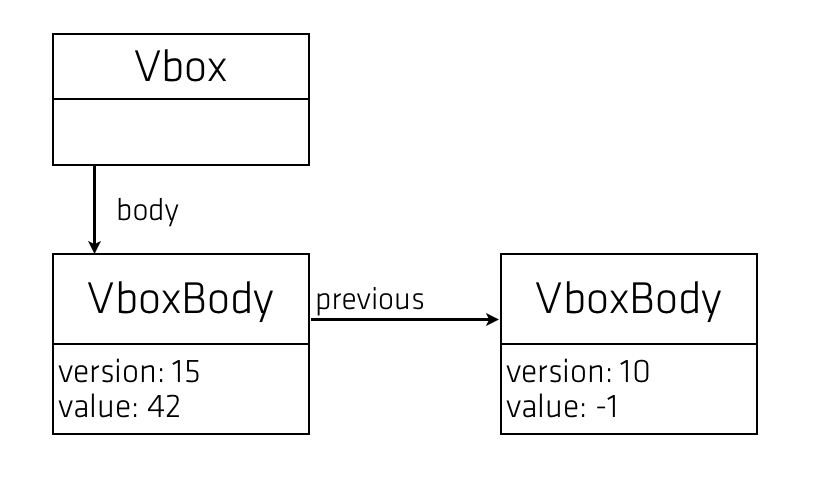
\includegraphics[width=0.5\linewidth]{vbox-list}
\caption{VBox Structure}
\label{fig:vbox}
\end{figure}

A Fenix Framework VBox however, also contains a back-pointer to its
owner, as well as the name of the slot it represents. This allows for
the persistence support to know where to store the value of the Box.

Those specialised VBoxes can have their previous values
Garbage-Collected and reloaded from persistent support on-demand.

\subsubsection{VBoxes for slots}

There are two layouts when mapping VBoxes in DomainObject slots: 1)
Using one VBox to keep the entire state of the object (One-Box) and 2)
Using one VBox per slot (Multi-Box).

The first layout suffers from a higher number of conflicts, as reading
one slot will conflict with writing another slot on the same object
(as they are mapped to the same VBox), however the memory usage is
much lower, as each VBox has a cost for its underlying data
structures. This aspect is critical in applications with a dense
domain model, with many objects and many slots.

Smaller applications can use the Multi-Box layout to greatly reduce
conflicts. In this layout, each domain slot is given its own VBox.

In both layouts, a specialised VBox called {\it PrimitiveBox} is
used to store either the object's state or the slot's value. There is
no added behaviour or data in a PrimitiveBox, however persistence
support uses this information to determine whether to reload a box
containing the state (or part of it) of an object or a box for a relation.

\subsubsection{VBoxes for relations}

In the One-Box layout, to-one relations are kept inside the object's
state, and as such require no special handling. 

On the other hand, for a Multi-Box layout, the reference to the
related object is kept in a {\it ReferenceBox}. Just like a {\it
  PrimitiveBox}, it contains no extra behaviour or data, and serves
only as a marker for persistence support to know it has to load an
object reference.

To-many relations however, are handled in a very different manner. The
preferred approach is to use a B+Tree\footnote{See
  $http://en.wikipedia.org/wiki/B+_tree$} to store the objects on the
to-many side of the relation. For each to-many relation, a {\it
  ReferenceBox} is generated, containing a reference to the domain
object representing the B+Tree.

The Fenix Framework provides an implementation of persistent B+Trees
that doesn't use to-many relations (by design, so it can be used to
implement them). In this implementation, each node of the tree is a
domain object containing only a reference to its parent and its
sibling. Inner nodes use an immutable TreeMap wrapper to keep indexed
references to the nodes they point to. Leaf nodes follow the same
strategy, keeping the mapping between keys and the objects they point
to (In reality they can be used to point at anything, however for this
document we are only interested in B+Trees containing domain objects).

As a B+Tree is generically a key-value map, its usage can be twofold:
provide a simple way to implement to-many relations and provide
support for relations indexed by a slot of the related
object. Consider the previously presented {\it Course} example. In
this model, one Course has many Students. As such, there is a B+Tree
slot in the Course Base class, which contain the references to all the
students enrolled in that particular course.

In the usual scenario, the B+Tree contains a mapping between OIDs and
the respective target object (which is rather useless, as the Fenix
Framework provides a lightweight API to read an object by its OID).
Now consider a scenario where the set of students must be indexed by
student name. The B+Tree will now contain a mapping between the
student's name and the target student, allowing for indexed lookups of
students by name.

